\section*{Math 202a - HW1 - Dan Davison - \texttt{ddavison@berkeley.edu}}

\begin{mdframed}
  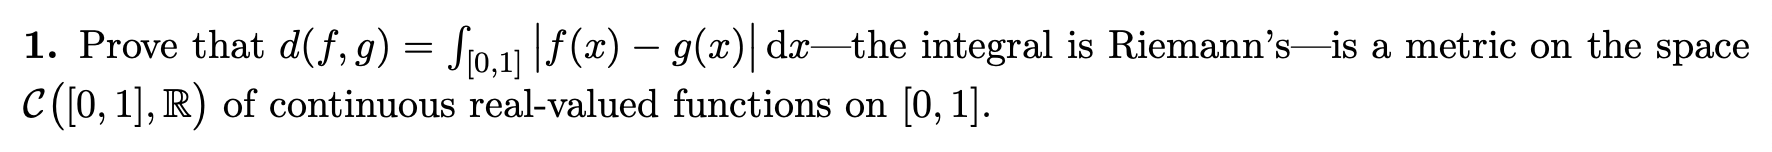
\includegraphics[width=400pt]{img/analysis--berkeley-202a--homework-1-a75a.png}
\end{mdframed}


\begin{proof}
  $d$ is a metric if it satisfies (I) $d(f,f) = 0$, (II) $d(f,g) = d(g, f)$, and (III) $d(f,g) + d(g, h) \le d(f, h)$.

  (I) is satisfied: $d(f, f) = \int_{[0,1]}|f(x) - f(x)| \dx = 0$.

  (II) is satisfied:
  \begin{align*}
    d(f, g)
    &= \int_{[0,1]}|f(x) - g(x)| \dx \\
    &= \int_{[0,1]}|g(x) - f(x)| \dx \\
    &= d(g, f),
  \end{align*}

  (III) is satisfied:
  \begin{align*}
    d(f, g) + d(g, h)
    &= \int_{[0,1]} |f(x) - g(x)| \dx + \int_{[0,1]} |g(x) - h(x)| \dx \\
    &= \int_{[0,1]} |f(x) - g(x)| + |g(x) - h(x)| \dx \\
    &\le \int_{[0,1]} |f(x) - g(x) + g(x) - h(x)| \dx \\
    &= \int_{[0,1]} |f(x) - h(x)| \dx \\
    &= d(f, h).
  \end{align*}
\end{proof}

\newpage
\begin{mdframed}
  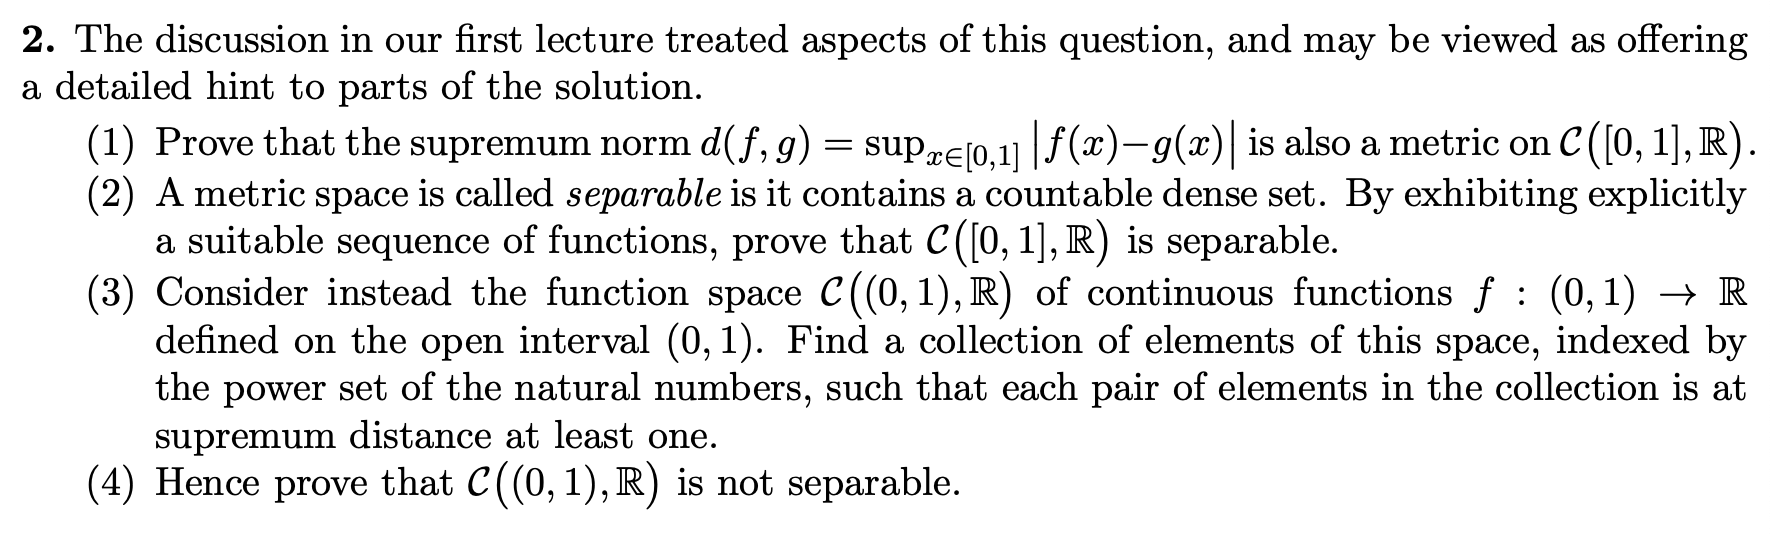
\includegraphics[width=400pt]{img/analysis--berkeley-202a--homework-1-d1d3.png}
\end{mdframed}

\begin{enumerate}
\item
  \begin{proof}
    $d$ is a metric on the function space $\mathcal C\([0, 1], \R\)$ if it satisfies (I) $d(f,f) = 0$,
    (II) $d(f,g) = d(g, f)$, and (III) $d(f,g) + d(g, h) \le d(f, h)$.

    (I) is satisfied: $\sup_{x\in [0,1]} |f(x) - f(x)| = \sup_{x\in [0,1]} 0 = 0$.

    (II) is satisfied:
    \begin{align*}
      d(f, g)
      &= \sup_{x \in [0,1]}|f(x) - g(x)| \\
      &= \sup_{x \in [0,1]}|g(x) - f(x)| \\
      &= d(g, f),
    \end{align*}
    (III) is satisfied:
    \begin{align*}
      d(f, g) + d(g, h)
      &=   \sup_{x \in [0,1]} |f(x) - g(x)| + \sup_{x \in [0,1]} |g(x) - h(x)| \\
      &=   \sup_{x \in [0,1]} \Big(|f(x) - g(x)| + |g(x) - h(x)|\Big) \\
      &\le \sup_{x \in [0,1]} |f(x) - h(x)| \\
      &=   d(f, h).
    \end{align*}
  \end{proof}
\item
  \begin{claim*}
    $\mc C\([0, 1], \R\)$ is separable.
  \end{claim*}

  \begin{proof}
    Let $\mc C$ be the set of continuous functions $[0, 1] \to \R$.

    Fix an arbitrary function $f \in \mc C$ and fix some $\epsilon > 0$.

    Define $g^*_n: [0, 1] \to \R$ as follows:
    \begin{enumerate}
    \item For all $i \in 0, 1, 2, \ldots, n$ set $x_i = i/n$.
    \item For all $i \in \{0, 1, 2, \ldots, n\}$, set $y^*_i = f(x_i)$. (Note that $y^*_i$ is in general not a rational
      number; we will account for this later.)
    \item For all $i \in \{1, 2, \ldots, n\}$ draw a straight line segment connecting $(x_{i-1}, y^*_{i-1})$
      and $(x_i, y^*_i)$.
    \item Define $g^*_n: [0, 1] \to \R$ to be the function whose graph was just drawn. (It is possible to give an
      explicit procedure for computing $g^*_n(x)$ by finding the interval in which $x$ lies and then using linear
      interpolation.)
    \end{enumerate}

    We now modify the definition of the family of approximating functions so that the $y$-coordinates of the
    endpoints are rational. Define $g_n: [0, 1] \to \R$ as follows:
    \begin{enumerate}
    \item Construct the sets of points $\{(x_i, y^*_i) ~|~ i \in \{0, 1, 2, \ldots, n\}\}$ as above.
    \item For $i \in \{0, 1, 2, \ldots, n\}$ set $y_i$ equal to a rational number in the
      interval $(y^*_i - \epsilon/4, y^*_i)$. (Such a rational number exists: for example, set $k$ equal to the
      smallest natural number such that $1/k < \epsilon/4$, and then set $j$ equal to the smallest natural number
      such that $j/k > y^*_i - \epsilon/4$. Then $j/k$ is a rational number in $(y^*_i - \epsilon/4, y^*_i)$.)
    \item For all $i \in \{1, 2, \ldots, n\}$ draw a straight line segment connecting $(x_{i-1}, y_{i-1})$
      and $(x_i, y_i)$.
    \item Define $g_n: [0, 1] \to \R$ to be the function whose graph was just drawn.
    \end{enumerate}
    Note that, since $f$ is continuous on a compact domain, $f$ is uniformly continuous. Fix some $\delta > 0$ such
    that $|x - x'| < \delta \implies |f(x) - f(x')| < \epsilon$ for all $(x, x') \in [0, 1]^2$.

    Set $m$ equal to the smallest natural number such that $1/m < \delta/2$ and note
    that $|f(x) - g_n(x)| < \epsilon$ for all $x \in [0, 1]$ due to the uniform continuity of $f$. (Informally,
    this is true because we can view uniform continuity as stating that a rectangle of base $\delta$ and
    height $\epsilon$ can be positioned over the graph at any point such that the graph intersects the left and
    right edges of the rectange but does not otherwise leave the rectangle. Our piecewise affine function
    consists of straight line segments that fit within such rectangles.) Therefore $d(g_n, f) < \epsilon$ for
    all $n \geq m$ and so $\{g_n | n \in \N\}$ is dense in $\mc C$.

    Finally we must show that $\{g_n ~|~ n \in \N\}$ is countable. Note that $g_n$ is piecewise affine for a
    given $n$, and that the $x$-coordinates of the endpoints are fixed. Thus for a given $n$, the cardinality
    of $\{g_n\}$ is equal to the cardinality of the set of possible $y$-coordinates. The latter set is $\Q^n$.
    Thus the cardinality of $\{g_n ~|~ n \in \N\}$ is equal to the cardinality of the
    set $\bigcup_{n\in \N} \Q^n$. This is a countable union of countable sets and is therefore countable.
  \end{proof}

\item
  \begin{proof}
    Let $f_s: (0, 1) \to \R$ be given by $f_s(x) = \frac{1}{r(s)x}$, where $s \in 2^\N$ and $r(s) \in [0, 1]$ is
    the real number corresponding to $s$, i.e. the number $r(s) = 0.d_1d_2d_3\ldots$ where
    \begin{align*}
      d_i =
      \begin{cases}
        1, ~~~~ \text{if} ~~~~ i \in s,\\
        0, ~~~~ \text{otherwise}.
      \end{cases}
    \end{align*}
    Note that for real $a, b$ we have
    \begin{align*}
      \frac{1}{ax} - \frac{1}{bx} = \frac{b - a}{abx}
    \end{align*}
    and therefore the supremum distance between any two elements $f_{s_1}$ and $f_{s_2}$ is unbounded
    as $x \to 0$.
  \end{proof}
\item
  \begin{proof}
    Let $\mc C$ be the set of continuous functions $f: (0, 1) \to \R$.

    Assume for a contradiction that $\mc C$ is separable. Let $\mc G \subset \mc C$ be a countable dense set of
    functions.

    Recall that in part (3) we found an uncountable set $\mc H \subset \mc C$ with the property that every pair
    of elements in $\mc H$ is at supremum distance at least one.

    But this is a contradiction, since we can establish a bijection between $\mc H$ and $\mc G$ as follows:

    Pick an element $h_1 \in \mc H$. Since $\mc G$ is dense in $\mc C$, there exists $g_1 \in \mc G$ such
    that $d(h_1, g_1) < 1/2$. Now pick $h_2 \in \mc H$ such that $h_1 \neq h_2$. Again, there
    exists $g_2 \in \mc G$ such that $d(h_2, g_2) < 1/2$. Furthermore, by the triangle
    inequality, $g_2 \neq g_1$. Continuing in this fashion, on the $i$-th iteration we pick $h_i \in \mc H$ and
    find a nearby $g_i \in \mc G$ such that $d(h_i, g_i) < 1/2$, and by the triangle inequality conclude
    that $g_i \neq g_j$ for all $j < i$.

    Thus we can associate each element of $\mc H$ with a unique element of $\mc G$ and conclude that the
    cardinality of $\mc G$ equals that of $\mc H$, which is that of the power set of the natural numbers.
    But $\mc G$ is countable; a contradiction. Therefore no such countable dense set $\mc G$ exists and $\mc C$
    is not separable.
  \end{proof}


  But can find bounded fns with image [0, 1]

  \begin{mdframed}
    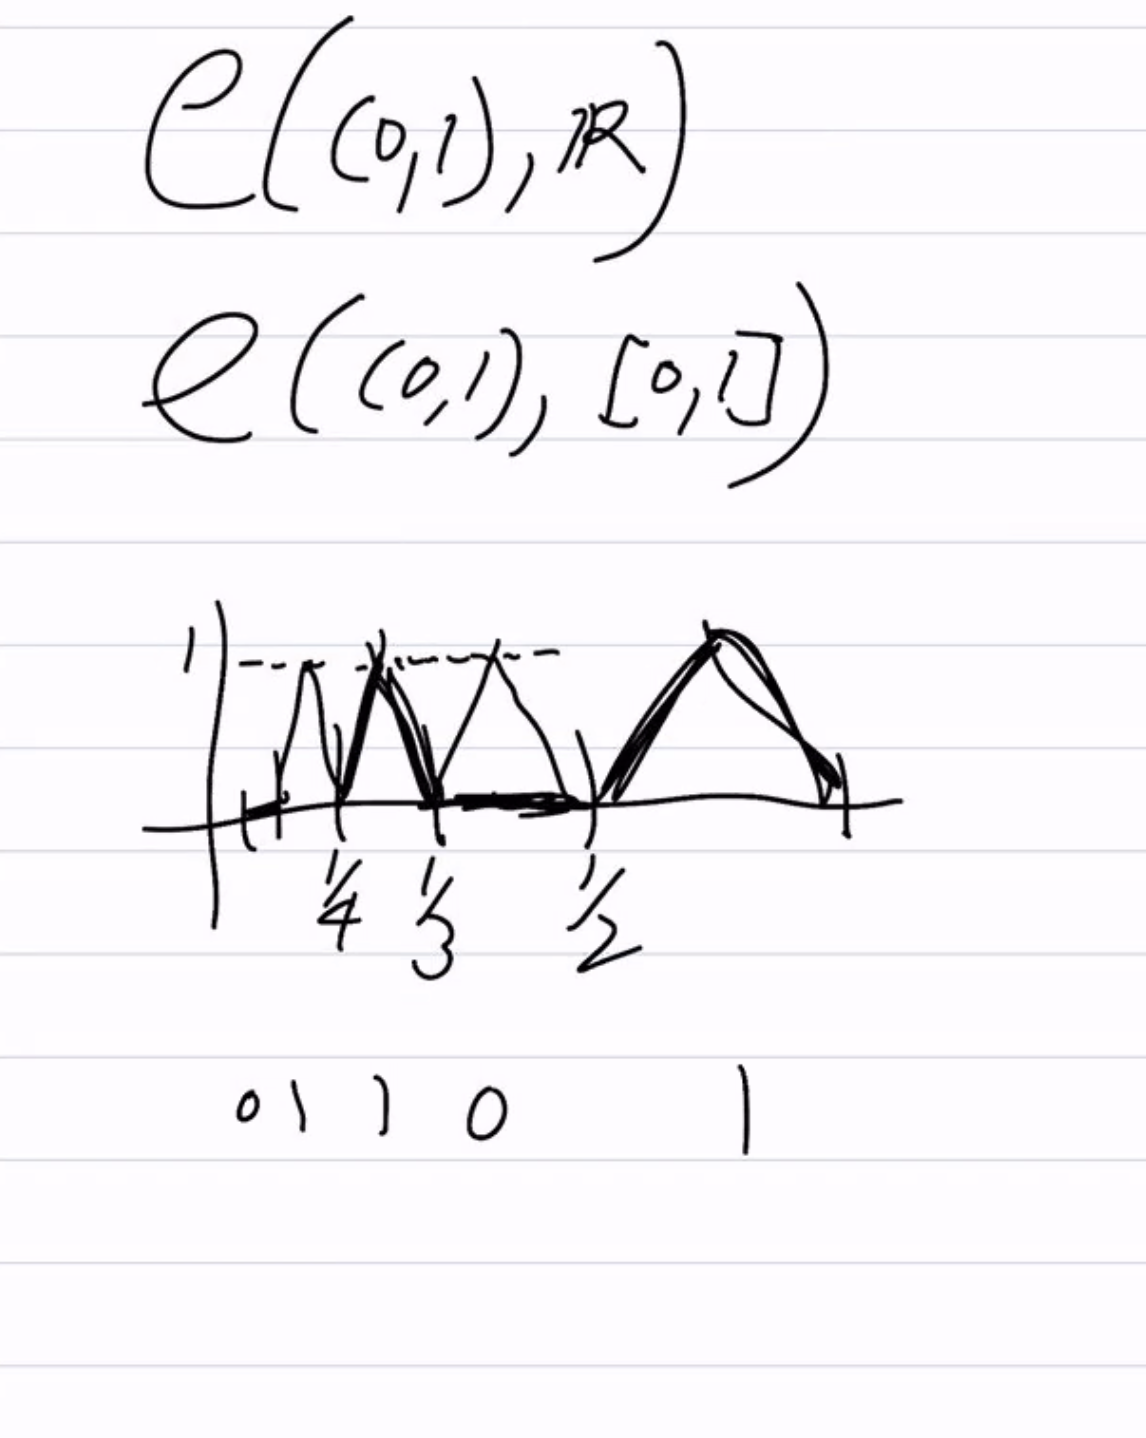
\includegraphics[width=400pt]{img/analysis--berkeley-202a-hw-7459.png}
  \end{mdframed}
\end{enumerate}


\newpage
\begin{mdframed}
  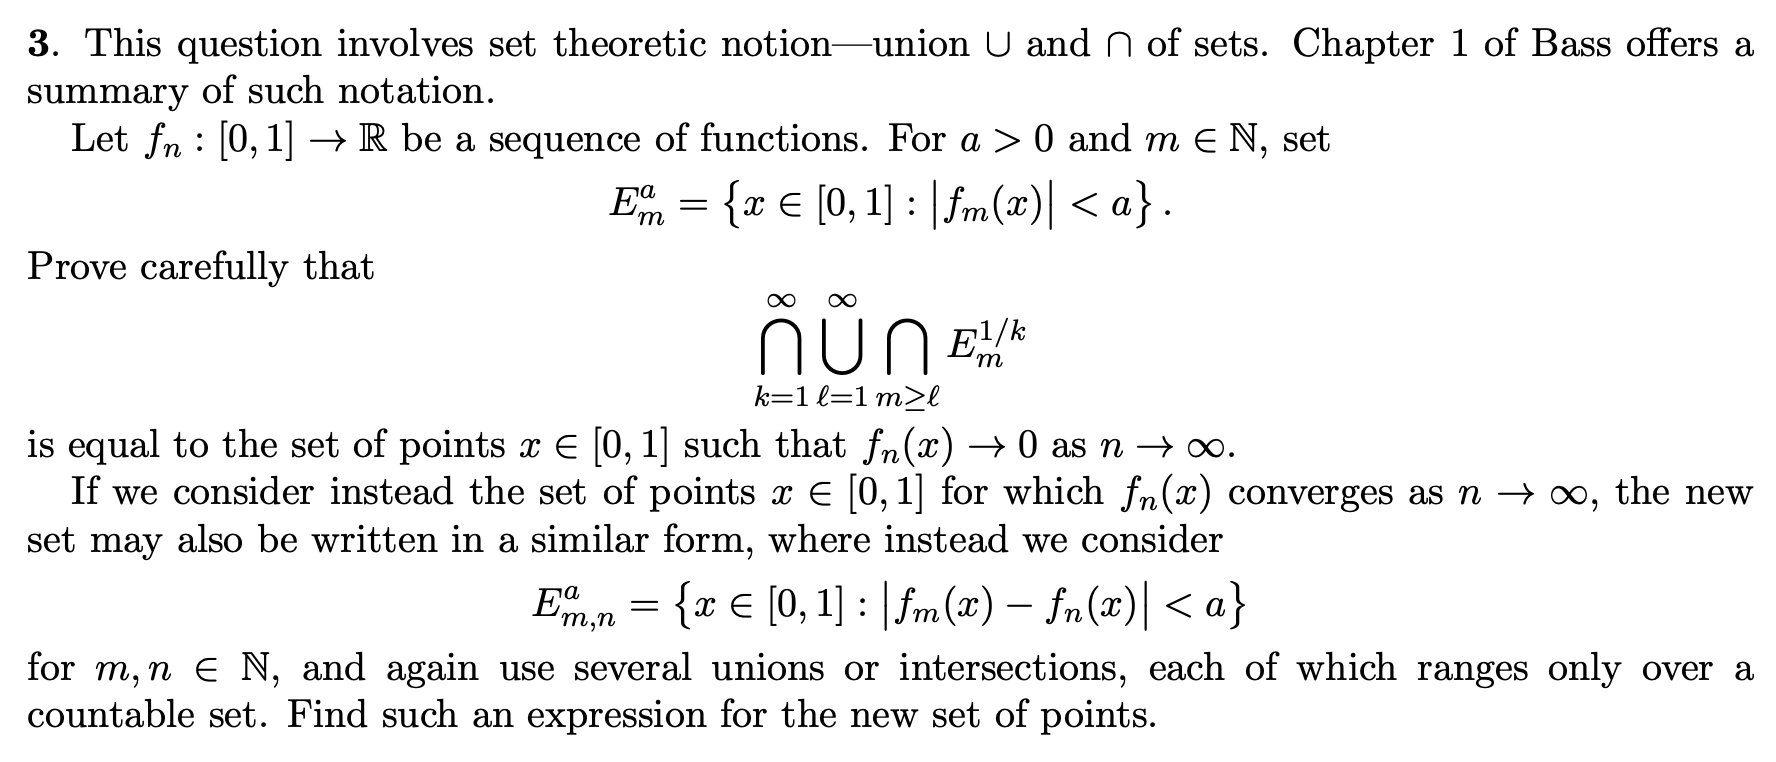
\includegraphics[width=400pt]{img/analysis--berkeley-202a--homework-1-8349.png}
\end{mdframed}


\begin{proof}
  Let $E_m^a = \{x \in [0, 1] : |f_m(x) < a|\}$ and let $T = \bigcap_{k=1}^\infty \bigcup_{l=1}^\infty \bigcap_{m > l} E_m^{1/k}$.

  Informally, $E_m^a$ is the set of points for which $f_m$ is within $a$ of zero.

  Let $f_n: [0, 1] \to \R$ be a sequence of functions and let $S \subseteq [0, 1]$ be the set of points $x$
  such that $f_n(x) \to 0$ as $n \to \infty$.

  First we prove that $x \in S \implies x \in T$.

  So let $x \in S$. Then from the definition of limit we have
  \begin{align*}
    &\forall \epsilon>0 ~~~~ \exists l \in \N ~~~~ \forall m \geq l ~~~~  x \in E_m^\epsilon \\
    \iff &\forall \epsilon>0 ~~~~ \exists l \in \N ~~~~                        x \in \bigcap_{m \geq l} E_m^\epsilon \\
    \iff &\forall \epsilon>0 ~~~~                                              x \in \bigcup_{l=1}^\infty \bigcap_{m \geq l} E_m^\epsilon \\
    \iff &                                                              x \in \bigcap_{k=1}^\infty \bigcup_{l=1}^\infty \bigcap_{m \geq l} E_m^{1/k} = T,
  \end{align*}
  as required.

  Secondly we prove that $x \in T \implies x \in S$.

  So let $x \in T$. We have
  \begin{align*}
    x \in \bigcap_{k=1}^\infty \bigcup_{l=1}^\infty \bigcap_{m \geq l} E_m^{1/k},
  \end{align*}
  which is equivalent to the statement
  \begin{align*}
    \forall k>0 ~~~~ \exists l \in \N ~~~~ \forall m \geq l ~~~~  |f_m(x)| < \frac{1}{k}.
  \end{align*}
  Let $\epsilon > 0$ be a real number. Then there exists $k \in \N$ such that $\frac{1}{k} < \epsilon$. Therefore we have
  \begin{align*}
    \forall \epsilon>0 ~~~~ \exists l \in \N ~~~~ \forall m \geq l ~~~~  |f_m(x)| < \epsilon
  \end{align*}
  which is equivalent to $x \in S$, as required.
\end{proof}

\begin{proof}
  Let $S \subseteq [0, 1]$ be the set of points $x$ for which $f_n(x)$ converges as $n \to \infty$. Since every
  convergent sequence in the reals is Cauchy, we have that $x \in S$ is equivalent to
  \begin{align*}
    \forall \epsilon > 0 ~~~~ \exists l \in \N ~~~~ \forall m \geq l ~~~~ \forall n \geq l ~~~~ |f_m(x) - f_n(x)| < \epsilon,
  \end{align*}
  which is equivalent to
  \begin{align*}
    \forall \epsilon > 0 ~~~~ x \in \bigcup_{l=1}^\infty \bigcap_{m \geq l} \bigcap_{n \geq l} E_{m,n}^\epsilon.
  \end{align*}
  Therefore, we have that $x \in S$ implies
  \begin{align*}
    x \in \bigcap_{k=1}^\infty \bigcup_{l=1}^\infty \bigcap_{m \geq l} \bigcap_{n \geq l} E_{m,n}^{1/k}.
  \end{align*}
  As before, the reverse implication also holds since, for any given $\epsilon > 0$, we can find a $k \in \N$
  such that $\frac{1}{k} < \epsilon$.
\end{proof}

\newpage
\begin{mdframed}
  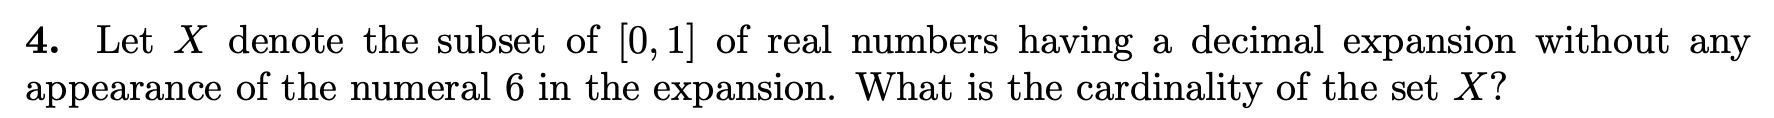
\includegraphics[width=400pt]{img/analysis--berkeley-202a--homework-1-f175.png}
\end{mdframed}


\begin{proof}
  Let $X \subset [0, 1]$ be the subset of real numbers without any 6 in their decimal expansion. Let $x \in X$ and let
  \begin{align*}
    d_n(x) =
    \begin{cases}
      0, ~~~~ n\text{-th decimal place of }x \text{ is }0\\
      1, ~~~~ \text{otherwise}.
    \end{cases}
  \end{align*}
  Define $f: X \to [0, 1]$ by setting $f(x)$ equal to the real number whose binary expansion
  is $0.d_1(x)d_2(x)\cdots$.

  Note that for any real number $\om \in [0, 1]$, there exists $x \in X$ such that $f(x) = \om$. To find such
  an $x$, we could for example choose the number whose decimal expansion is equal to the binary expansion
  of $\om$.

  Therefore $f$ is a non-injective surjection from $X$ to the reals in $[0, 1]$, and so the cardinality of $X$
  is at least that of the reals. Since $X \subset \R$ we conclude that the cardinality of $X$ is equal to that
  of the reals.
\end{proof}

\newpage
\begin{mdframed}
  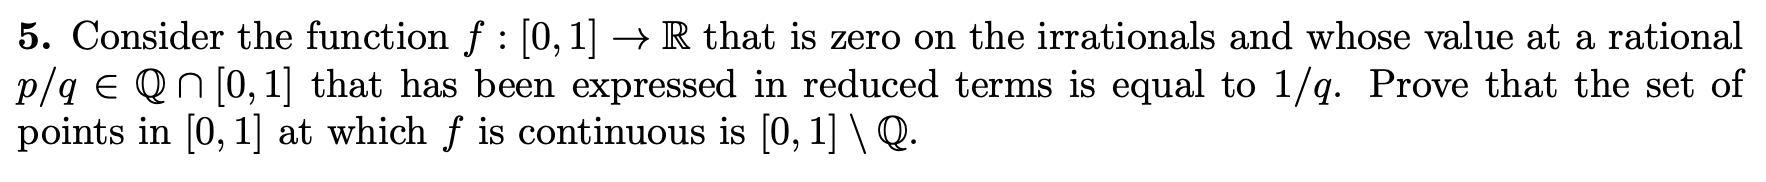
\includegraphics[width=400pt]{img/analysis--berkeley-202a--homework-1-5192.png}
\end{mdframed}



\begin{proof}
  Let $X \subseteq [0, 1]$ be the set of points at which $f$ is continuous. We want to show that $f$ is
  continuous at $x$ iff $x$ is not rational.

  Suppose for a contradiction that $f$ is continuous at a rational point $x = p/q$, where $p, q$ are
  non-negative integers. Then $f(x) = 1/q$. But there will always be irrational points within a given
  distance $\delta$ of $x$, now matter how small $\delta$ is, and at such an irrational point $x'$ we
  have $|f(x) - f(x')| = |1/q - 0| = 1/q$. Therefore $f$ is not continuous at $x$ since the definition of
  continuity does not hold for $\epsilon < 1/q$.

  Now let $x$ be irrational, so that $f(x) = 0$. Fix an arbitrary $\epsilon > 0$. We want to show that there
  exists a $\delta$ such that $1/q < \epsilon$ for any rational point $p/q$ lying within $\delta$ of $x$,
  where $p/q$ is in reduced terms. If $\epsilon > 1/2$ then any $\delta$ will work, so
  assume $\epsilon \leq 1/2$. Let $k$ be the largest natural number such that $1/k \geq \epsilon$, let $i$ be
  the largest natural number such that $i/k < x$ and let $j$ be the smallest natural number such
  that $j/k > x$. Then a choice of $\delta = \frac{1}{2}\min\{x - i/k, j/k - x\}$ will work to prove continuity
  of $f$ at irrational $x$.
\end{proof}


\begin{mdframed}
  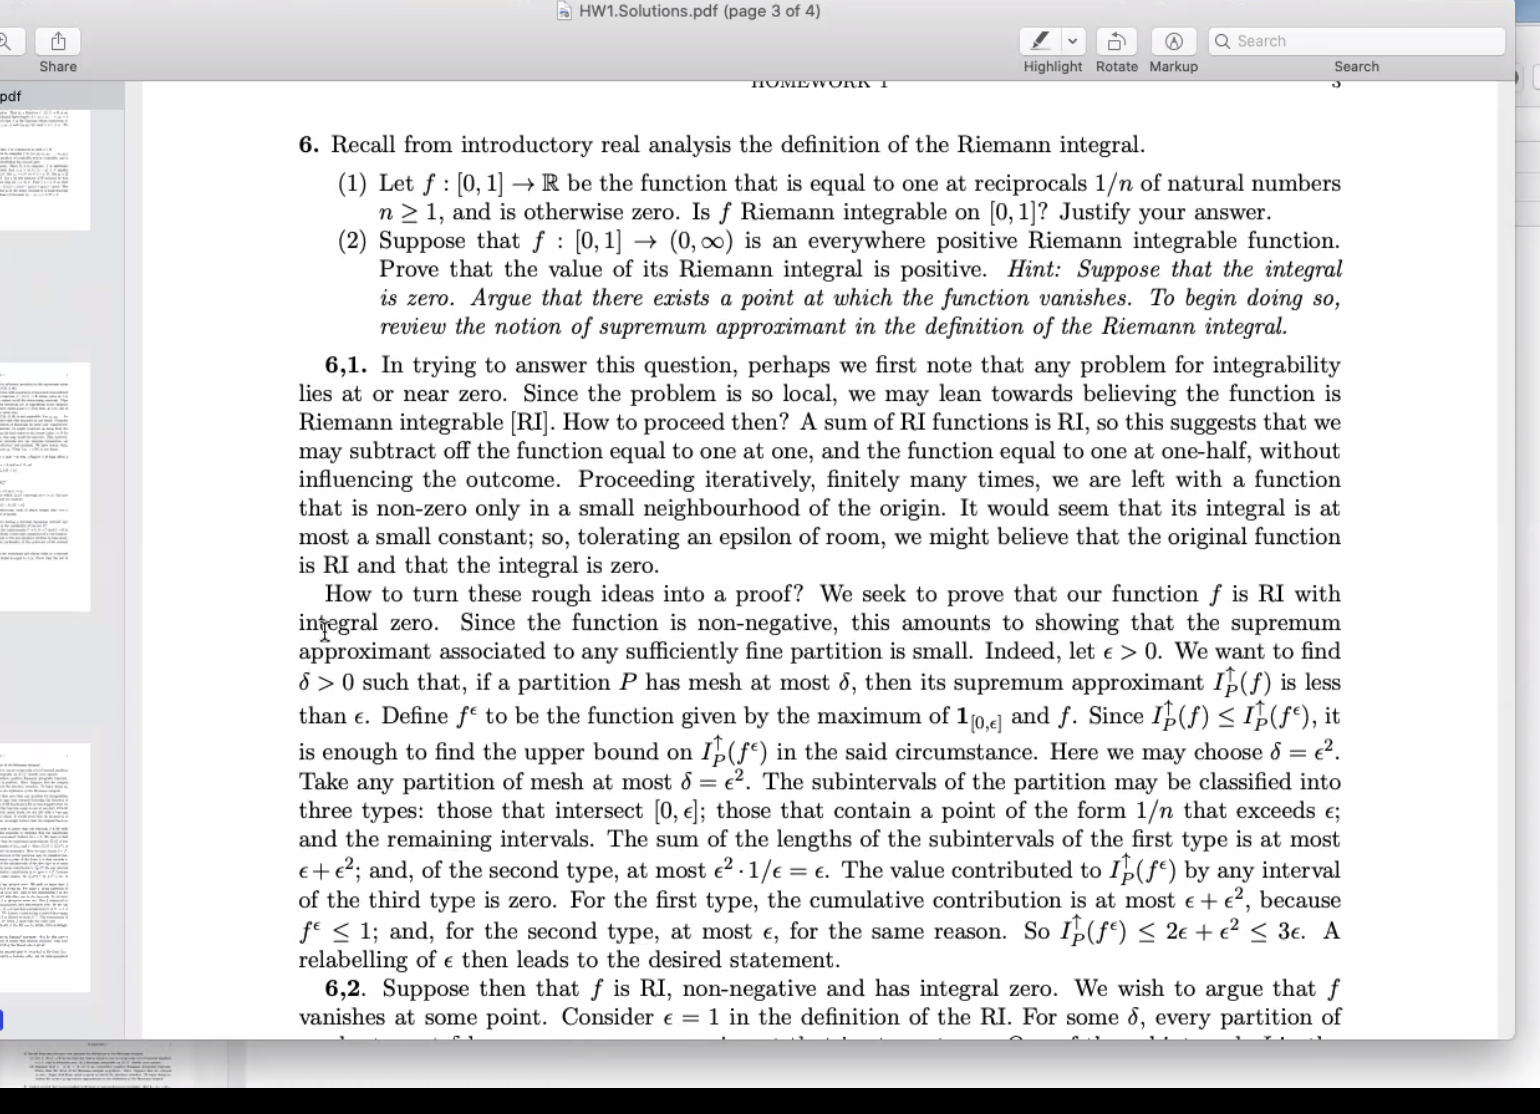
\includegraphics[width=400pt]{img/analysis--berkeley-202a-hw-af4c.png}
\end{mdframed}


\begin{mdframed}
  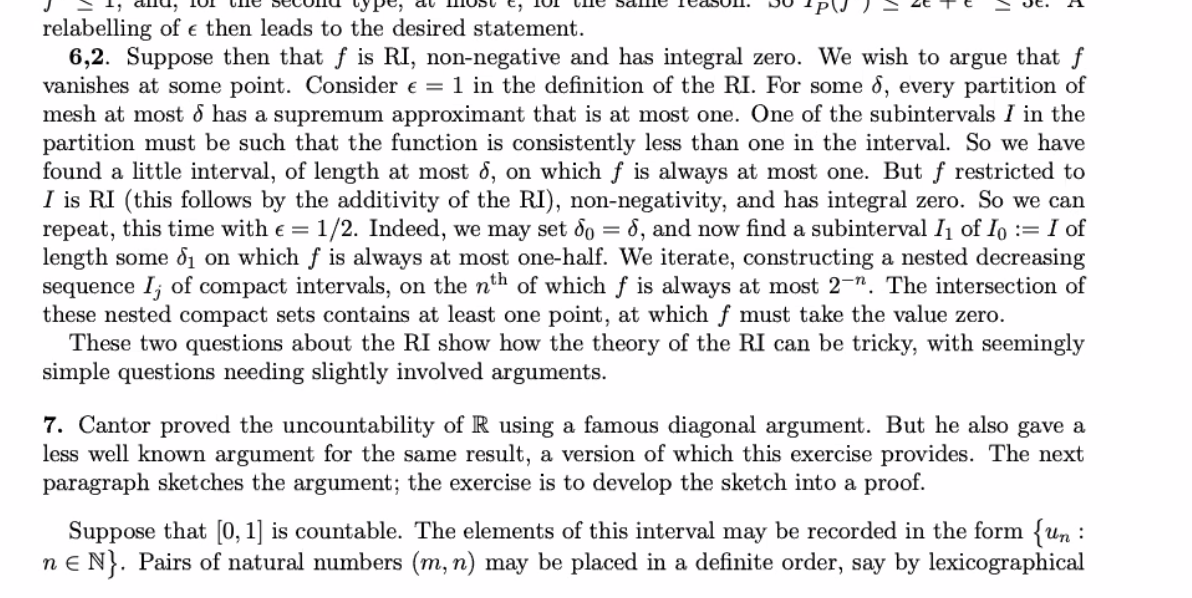
\includegraphics[width=400pt]{img/analysis--berkeley-202a-hw-5fee.png}
\end{mdframed}




\newpage
\begin{mdframed}
  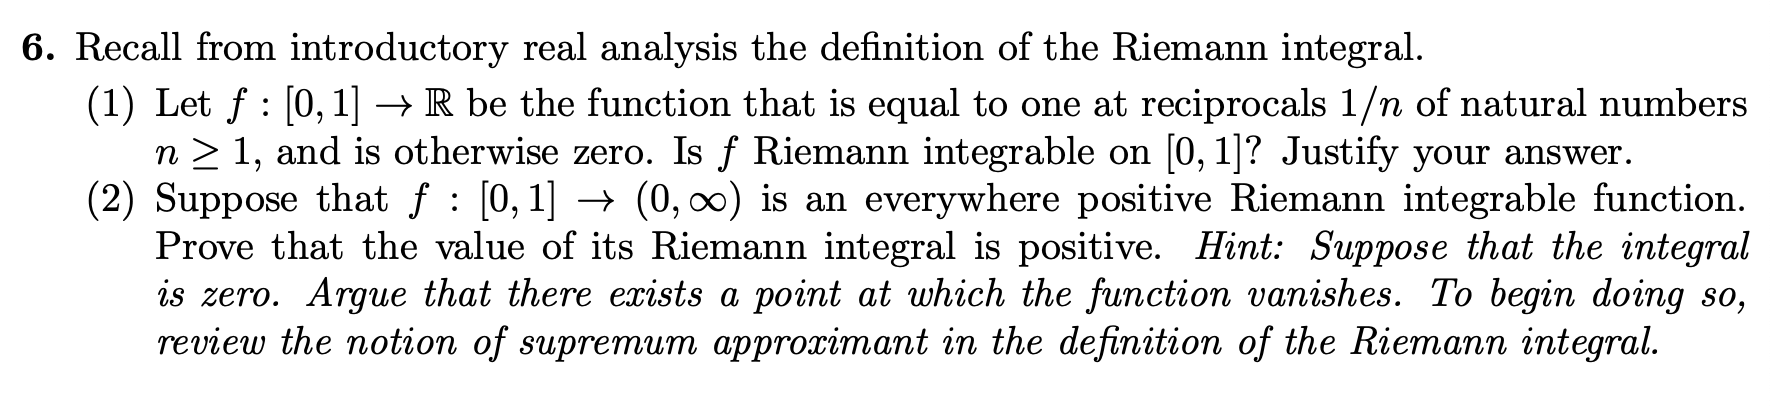
\includegraphics[width=400pt]{img/analysis--berkeley-202a--homework-1-f5e8.png}
\end{mdframed}





\begin{definition*}
  $g: [0, 1] \to \R$ is Riemann integrable if
  \begin{align*}
    \sup_{\phi^-} I(\phi^-) = \inf_{\phi^+} I(\phi^+).
  \end{align*}
  Here $\phi^-$ and $\phi^+$ are step functions adapted​ to some
  partition $0 \leq x_1 \leq x_2 \leq \ldots \leq x_{n-1} \leq 1$, such that $\phi(x) = c_i$
  for $x \in (x_{i-1}, x_i)$. $I(\phi)$ is (informally) the area under the step function $\phi$:
  \begin{align*}
    I(\phi) = \sum_{i=1}^n c_i(x_i - x_{i-1}).
  \end{align*}
  And the supremum is over all minorants $\phi^- \leq g$ and the infimum is over all
  majorants $\phi^+ \geq g$, where the length $n$ of the partition is allowed to vary as well as the constant
  values $\{c_1, c_2, \ldots, c_n\}$ of the step function within each segment.
\end{definition*}

\begin{enumerate}
\item
  \begin{claim*}
    The specified function $f$ is not Riemann integrable.
  \end{claim*}

  \begin{proof}
    Consider the first segment of any partition: $(0, x_1)$. No matter how small $x_1$ is, there
    exists $n \in \N$ such that $1/n < x_1$. Therefore for all majorants we have $c_1 \geq 1$ and yet for all
    minorants we have $c_1 \leq 0$. So, when restricted to this first segment, we have $I(\phi^-) > I(\phi^+)$
    for all $\phi^-, \phi^+$ and, since every majorant is elsewhere less than every minorant, it is not
    possible that $\sup_{\phi^-} I(\phi^-) = \inf_{\phi^+} I(\phi^+)$ and hence the Riemann integral is
    undefined.
  \end{proof}

\item
  \begin{claim*}
    $\int_0^1 f > 0$
  \end{claim*}
  \begin{proof}
    Suppose for a contradiction that $\int_0^1 f = 0$. Fix an arbitrary minorant $\phi^-$, adapted to a
    partition of length $n$. Then we have that $\sum_{i=1}^n c_i(x_i - x_{i-1}) \leq 0$.
    Since $x_i \geq x_{i-1}$ for all $i$, and since $x_0 = 0 < x_n = 1$, it must be the case
    that $x_i - x_{i-1} > 0$ for some $i$, and therefore that $c_i > 0$ for some $i$. Therefore $f$ vanishes at
    at least one point. This contradiction proves that $\int_0^1 f \neq 0$.

    To see that it's not negative, note that for every majorant $\phi^+$ we have $x_i - x_{i-1} \geq 0$
    and $c_i > 0$ for all $i$ and therefore $I(\phi^+) = \sum_{i=1}^n c_i(x_i - x_{i-1}) \geq 0$. Therefore $\int_0^1 f > 0$.
  \end{proof}

\end{enumerate}

\newpage
\begin{mdframed}
  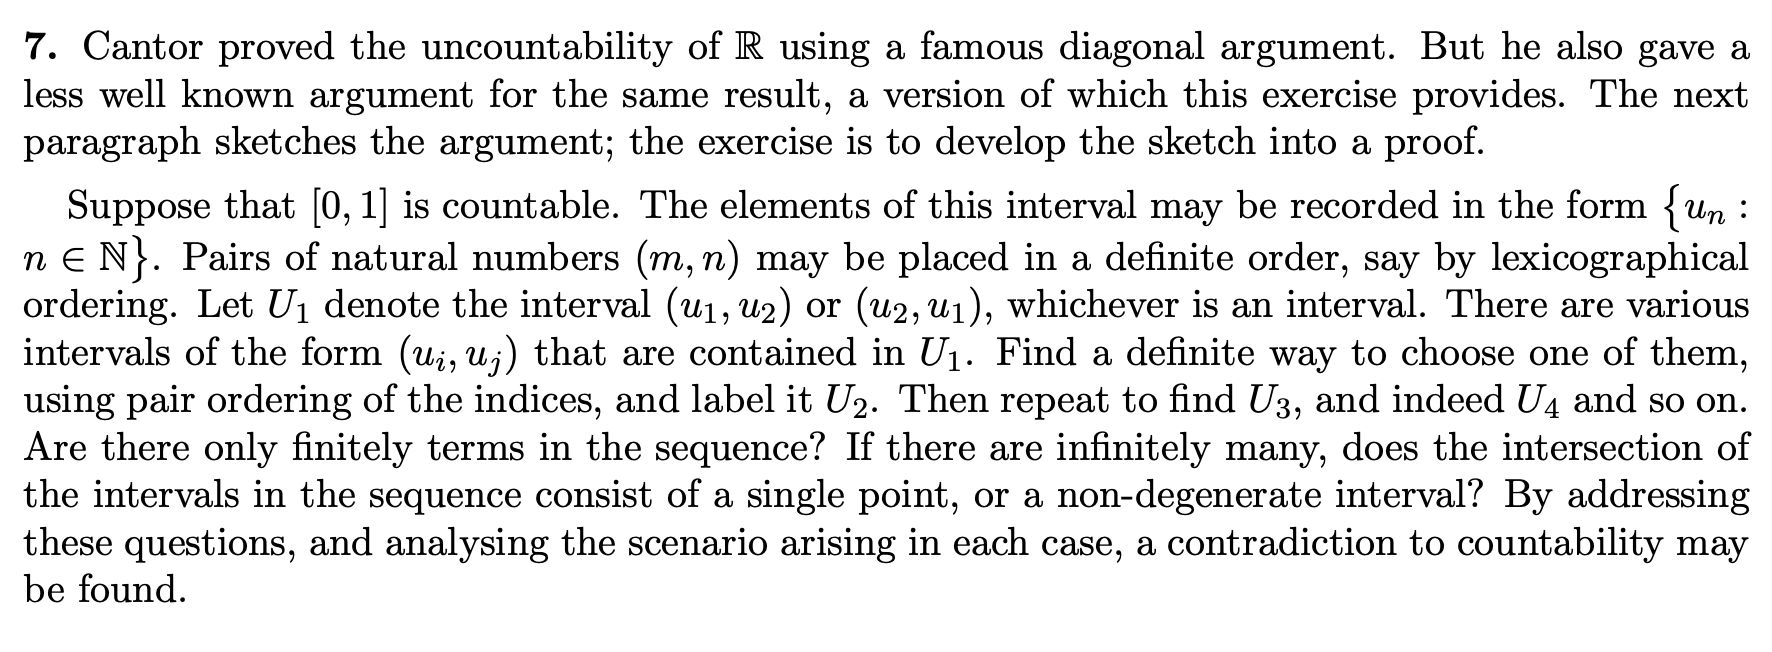
\includegraphics[width=400pt]{img/analysis--berkeley-202a--homework-1-a577.png}
\end{mdframed}

\begin{proof}
  Suppose for a contradiction that $[0, 1] \subset \R$ is countable. Fix an enumeration $\{u_n ~|~ n \in \N\}$
  of the elements of $[0, 1]$.

  If $u_1 > u_2$ then relabel them so that $u_1 < u_2$. Set $U_1 = (u_1, u_2)$.

  Continue examining the numbers in the enumeration (starting at $u_3$) until two numbers have been encountered
  that are both in $(u_1, u_2)$. Form an interval from this pair and label it $U_2$. Continue examining the
  numbers in the enumeration until two numbers are encountered that are both in $U_2$; label this
  interval $U_3$. Continue in this fashion indefinitely.

  We will write $(U_{i1}, U_{i2})$ to refer to the endpoints of interval $i$.

  There are two cases:

  \begin{enumerate}
  \item {\bf The process terminates.}\\
    Then there is a last interval $U_L = (U_{L1}, U_{L2})$. It is possible that there is one (but not more than
    one) element $u^*$ of the original enumeration that is present in the interval $U_L$. If that is so, then
    every element of $U_L \setminus \{u^*\}$ is a real number not in the original enumeration; otherwise every
    element of $U_L$ is a real number not in the original enumeration.

  \item {\bf The process does not terminate.}\\
    Note that the sequence of interval lower bounds $(U_{i1})_{i\in\N}$ forms a strictly increasing sequence
    bounded above by $u_2$ and that the sequence of interval upper bounds $(U_{i2})_{i\in\N}$ forms a strictly
    decreasing sequence bounded below by $u_1$. By the Monotone Convergence theorem, both sequences converge:
    let these limits be $\alpha$ and $\beta$ respectively. There are two cases:
    \begin{enumerate}
    \item {\bf $\alpha < \beta$}\\
      Then every element of $(\alpha, \beta)$ is a real number not in the original enumeration.
    \item {\bf $\alpha = \beta$}\\
      Then $\alpha$ is a real number not in the original enumeration.
    \end{enumerate}
  \end{enumerate}

  In all cases, we found a real number that was not present in the original enumeration. But this is a
  contradiction, since the original enumeration contains all real numbers. Therefore no such enumeration exists
  and the real numbers are not countable.
\end{proof}
